Sia data la matrice di \textit{Toeplitz} simmetrica
\begin{equation}
     \label{eq:toeplitz}
     \begin{gathered}
          A_\mathrm{N}=\begin{pmatrix}
          4  & -1     &        & -1     &        &    \\
          -1 & \ddots & \ddots &        & \ddots &    \\
             & \ddots & \ddots & \ddots &        & -1 \\
          -1 &        & \ddots & \ddots & \ddots &    \\
             & \ddots &        & \ddots & \ddots & -1 \\
             &        & -1     &        & -1     & 4
          \end{pmatrix} \in\mathbb{R}^{NxN}, N\geq10,
     \end{gathered}
\end{equation}
in cui le extra-diagonali più esterne sono le none. Partendo dal vettore $\textbf{u}_\mathrm{0} = (1,...,1)^{T} \in \mathbb{R}^{N} $, applicare il metodo delle potenze con tolleranza $tol = 10^{-10}$ per $N = 10 : 10 : 500$, utilizzando la function del precedente esercizio. Graficare il valore dell'autovalore dominante, e del numero di iterazioni necessarie per soddisfare il criterio di arresto, rispetto ad $N$. Utilizzare la function \textbf{spdiags} di Matlab per creare la matrice e memorizzarla come matrice sparsa.

\hspace*{\fill}
\par\noindent\rule{\textwidth}{0.4pt}
\hspace*{\fill}
\begin{lstlisting}[language=Matlab, caption=Codice Matlab]
x = linspace(10, 500, 50);
ax1 = subplot(2, 1, 1);
ax2 = subplot(2, 1, 2);
l = zeros(50, 1);
it = zeros(50, 1);
tol = 1E-10;
for n = 10 : 10 : 500
     u = ones(n, 1);
     S = spdiags(u * [-1 -1 4 -1 -1], [-9, -1 : 1, 9], n, n);
     [l1, x1, i] = mypower(S, u, tol);
     l(n / 10) = l1;
     it(n / 10) = i;
end
plot(ax1, x, l);
plot(ax2, x, it);
legend(ax1, 'Autovalori dominanti');
legend(ax2, 'Iterazioni');
\end{lstlisting}
Le seguenti figure mostrano gli autovalori dominanti e le iterazioni necessarie al metodo delle potenze, al variare della dimensione della matrice  $A_\mathrm{N}$ con $N = 10 : 10 : 500$:
\begin{figure}[H]
     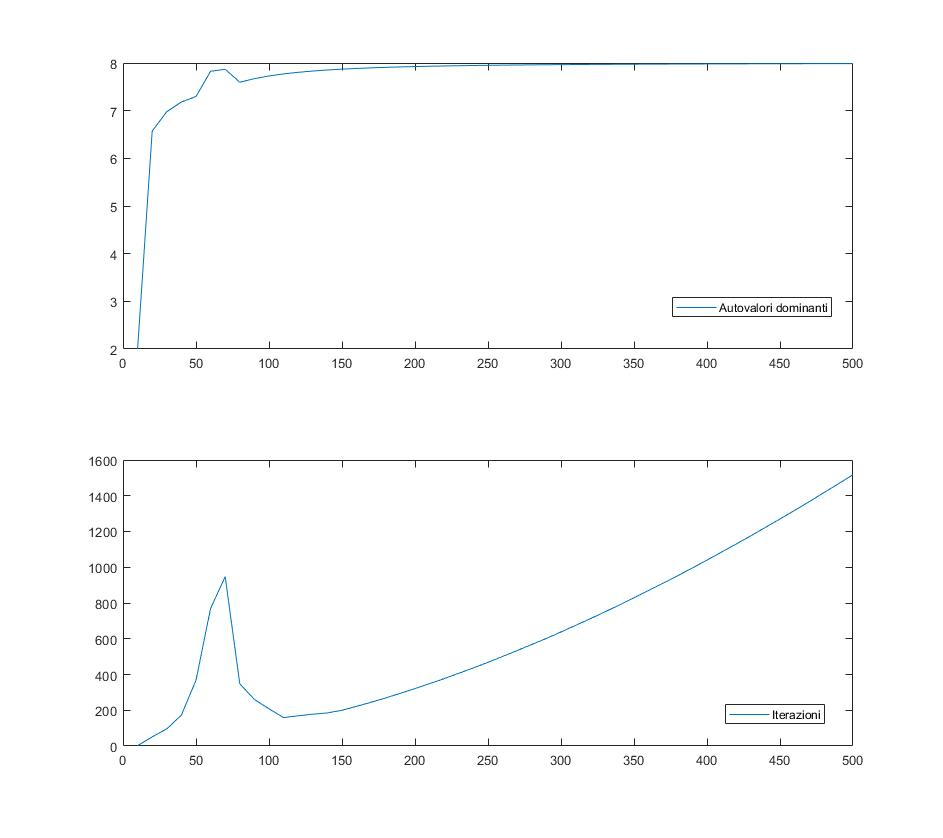
\includegraphics[width=\textwidth]{Chapter-6/Exercise-25/plot.jpg}
     \caption*{Autovalori dominanti e iterazioni del metodo delle potenze con $N = 10 : 10 : 500$}
\end{figure}
